\documentclass[11pt,a4paper]{article}
\usepackage[utf8]{inputenc}
\usepackage[british]{babel}
\usepackage[a4paper,margin=2.3cm]{geometry}
\usepackage{amsmath,amssymb}
\usepackage{graphicx}
\usepackage{tikz}
\usetikzlibrary{calc,angles,quotes,patterns}
\usepackage[most]{tcolorbox}
\usepackage{enumitem}
\usepackage{array}
\usepackage{titlesec}
\usepackage[hidelinks]{hyperref}

\definecolor{bandgreen}{RGB}{46,139,87}
\definecolor{bandblue}{RGB}{30,100,190}
\definecolor{bandamber}{RGB}{220,140,20}
\definecolor{bandpink}{RGB}{210,70,140}
\definecolor{bandpurple}{RGB}{110,50,160}

\newcounter{prob}
% \prob{label}{title}{source}
\newcommand{\prob}[3]{\par\bigskip\refstepcounter{prob}\label{#1}%
  \noindent\textbf{\theprob.\ #2}\hfill{\small\textit{#3}}\par\nopagebreak\smallskip}
\newcommand{\ans}[2]{\par\smallskip\noindent\textbf{\ref{#1}.}\ #2}

\newcommand{\band}[3]{%
  \clearpage
  \begin{tcolorbox}[colback=#1!12,colframe=#1,boxrule=1pt,arc=2pt]
  {\Large\bfseries\color{#1} #2}\hfill{\large #3}
  \end{tcolorbox}}

\newtcolorbox{diarynote}[1]{colback=black!4,colframe=black!45,boxrule=0.6pt,
  arc=2pt,fonttitle=\bfseries\small,title={#1},fontupper=\small}

\setlength{\parindent}{0pt}
\setlength{\parskip}{3pt}
\definecolor{bandgrey}{RGB}{85,85,85}
\begin{document}

\begin{titlepage}
\centering
\vspace*{3cm}
{\Huge\bfseries The Ladies' Diary for 1780\par}
\vspace{0.6cm}
{\Large One issue, ten problems\par}
\vspace{2cm}
{\large\itshape Fair Phillida sighs for---and sighs for in vain;\\
Ye fair-ones, oh pity her woes;\\
And from those equations the object explain,\\
That so greatly disturbs her repose.\par}
\vspace{0.3cm}
{\small Stephen Roberts, question 757\par}
\vfill
{\large Working draft\par}
\end{titlepage}

\section*{A word before the problems}

This booklet is made from a single almanac: \textit{The Ladies' Diary} for the year 1780,
number 77, printed for the Company of Stationers. Letters for it were to be addressed
``For the Ladies' Diary, Stationers' Hall, London''. Its editor at the time was Charles
Hutton, professor of mathematics at the Royal Military Academy, Woolwich.

An issue had two halves. The first half printed the answers to the questions set a year
earlier, here numbers 742 to 756. The second half set fifteen new ones, numbers 757 to
771, whose answers would appear in 1781. So a single issue never holds a question
together with its answer. For the answered questions we have the solvers' working but
not the original wording, and we have retold them from the working. For the new questions
we have the wording, and the answers here are our own.

The issue gives a fair picture of who was writing in. Mrs Eleanor Suggett is among the
solvers of the first, second and fifth questions. The two prizes for the prize enigma went
to Mrs Jane Roberts (ten free copies of the Diary) and Miss Diana Browne (eight). Mrs
Roberts also set a rebus and answered the rebuses of others. The prize question was set
by ``Peter Puzzlem'', who was John Landen. Among those who solved it was a Mr Wm.\
Herschel. This was William Herschel, then an organist at Bath. In March 1781 he
discovered the planet Uranus. His biographer, Edward Holden, counted the Diary answer as
his earliest published writing.\footnote{E.~S.~Holden, \textit{Sir William Herschel, his
Life and Works} (1881). Holden dates it by the question, 1779; the answer is printed in
the Diary for 1780, pp.~45--47.} Problem~\ref{y-string} is a version of his question.

\subsection*{How to read the labels}

\textit{Q743} is the Diary's own question number. Leybourn's collected edition keeps
these numbers. \textit{After Q743} means the question has been retold: we have changed the
numbers, or rebuilt the wording from the answers printed in 1780. The answer at the back
is then for the retelling. Pence and pints stay in problem~\ref{y-wine}, because the
problem is about them. Feet stay in problem~\ref{y-bird}, because the Diary's value of
gravity is in feet.

The bands are those of the first book in this series. The issue has nothing young
enough for Green. The last section, Beyond A-level, takes the mechanics and the hardest
of the series.

\subsection*{How this edition was made}
This edition was prepared with the assistance of Claude, an AI model made by Anthropic.
Under the editor's direction, Claude worked from a machine-read text of the 1780 issue.
It drafted the retellings, solutions, notes and introduction, recomputed every answer,
and typeset the text. Selection, editorial decisions and final responsibility for the
text are the editor's.

%================ BLUE ================
\band{bandblue}{Blue}{ages 8--11}

\prob{y-loaves}{Ali's loaves}{the arithmetical paradox, answered 1780}
Two travellers sit down to eat. One has 5 loaves and the other has 3. A stranger joins
them, and the three share the 8 loaves equally. When he leaves, the stranger puts down 8
pieces of money for his meal. The man with 5 loaves offers the other 3 pieces. The man
with 3 loaves says he should have half. They take it to the judge, Ali. Ali gives the
man with 3 loaves just 1 piece, and the other man 7. Was Ali fair?

%================ AMBER ================
\band{bandamber}{Amber}{ages 11--14}

\prob{y-wine}{The wine bill}{after Q746}
A man buys some pints of wine at 8 pence a pint and some at 5 pence a pint. The bill, in
pence, is a square number. If 360 is added to the bill, the result is the square of the
total number of pints. How many pints of each did he buy?

\prob{y-hobbes}{Hobbes's golden section}{after Q747}
Cut a line 2 units long into two parts so that the whole is to the longer part as the
longer part is to the shorter. Euclid's construction makes the longer part $\sqrt5-1$.
The Diary asked its readers to show that a construction it credits to Hobbes was wrong.
That construction makes the longer part $\sqrt{5-2\sqrt3}$. On a calculator the two
agree to two decimal places. Show, without a calculator, that they are not equal.

%================ PINK ================
\band{bandpink}{Pink}{ages 14--16}

\prob{y-circles}{Twice the chord}{after Q764, by the Rev.~Mr Lawson}
Two circles have radii 13 and 10, and their centres $O_1$ and $O_2$ are 26 apart. $P$ lies
on $O_1O_2$, 10 from $O_1$. A straight line through $P$ cuts both circles. At what angle
to $O_1O_2$ must it be drawn, so that its chord in the larger circle is twice its chord in
the smaller?

\begin{center}
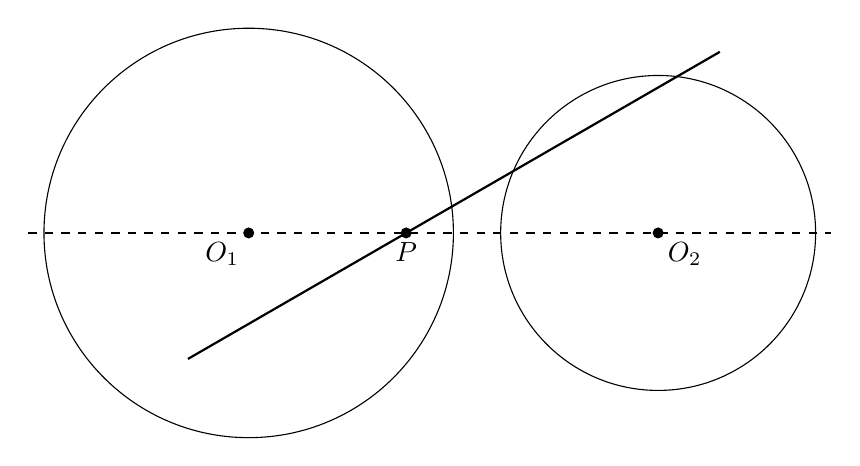
\begin{tikzpicture}[scale=0.2]
\coordinate (O1) at (0,0); \coordinate (O2) at (26,0); \coordinate (P) at (10,0);
\draw (O1) circle (13); \draw (O2) circle (10);
\draw[dashed] (-14,0) -- (37,0);
\draw[thick] ($(P)+(210:16)$) -- ($(P)+(30:23)$);
\fill (O1) circle (0.35) node[below left] {$O_1$};
\fill (O2) circle (0.35) node[below right] {$O_2$};
\fill (P) circle (0.35) node[below] {$P$};
\end{tikzpicture}
\end{center}

%================ PURPLE ================
\band{bandpurple}{Purple}{ages 16--17}

\prob{y-triangle}{The largest triangle}{after Q743}
In a triangle $ABC$, the perpendicular from $C$ meets $AB$ at $D$, between $A$ and $B$.
We know that $AC + AD = 26$ and $BC + BD = 37$. Find the sides of the triangle when its
area is as large as possible.

\begin{center}
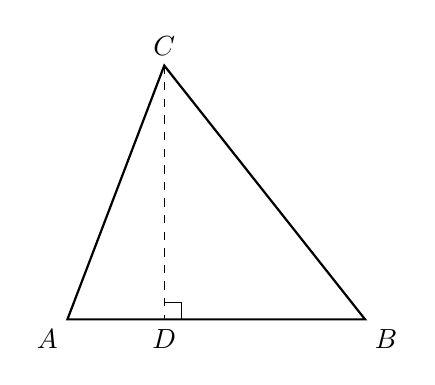
\begin{tikzpicture}[scale=0.18]
\coordinate (A) at (0,0); \coordinate (B) at (21,0);
\coordinate (D) at (6.833,0); \coordinate (C) at (6.833,17.907);
\draw[thick] (A) -- (B) -- (C) -- cycle;
\draw[dashed] (C) -- (D);
\draw (D) ++(0,1.2) -- ++(1.2,0) -- ++(0,-1.2);
\node[below left] at (A) {$A$}; \node[below right] at (B) {$B$};
\node[above] at (C) {$C$}; \node[below] at (D) {$D$};
\end{tikzpicture}
\end{center}

\prob{y-line}{The line through a point}{after Q766, by Thomas Moss}
A triangle has corners $C(0,0)$, $A(16,0)$ and $B(0,12)$, and $E$ is the point $(1,3)$
inside it. A straight line through $E$ meets $CA$ at $G$ and $CB$ at $H$. From $G$ and
$H$, perpendiculars $GM$ and $HN$ are drawn to $AB$. Where must the line go so that
$GM + HN$ is as long as possible? How long is it then?

%================ BEYOND ================
\band{bandgrey}{Beyond A-level}{motion and series}

\prob{y-slides}{Two slides, one time}{after Q744}
$C$ is 6\,m directly above $B$. Take $B$ as the origin, so that $C$ is $(0,6)$. The
point $A$ is $(5,1)$. A smooth straight wire runs from $C$ to $A$. Find the point $F$ on
$CA$ such that a bead sliding from rest straight from $F$ to $B$ takes exactly as long as
a bead sliding from rest from $C$ to $A$. How long do both take? Use $g = 9.8$\,m\,s$^{-2}$.

\begin{center}
\begin{tikzpicture}[scale=0.55]
\coordinate (B) at (0,0); \coordinate (C) at (0,6); \coordinate (A) at (5,1);
\coordinate (F) at (4,2);
\draw[thick] (C) -- (A); \draw[thick] (F) -- (B);
\draw[dashed] (B) -- (C);
\draw[gray,dotted] (-5.5,0) -- (5.5,0);
\fill (B) circle (0.07) node[below left] {$B$};
\fill (C) circle (0.07) node[above left] {$C$};
\fill (A) circle (0.07) node[right] {$A$};
\fill (F) circle (0.07) node[above] {$F$};
\end{tikzpicture}
\end{center}

\prob{y-bird}{The stone and the sea-mew}{Q761, by John Willes of Marske}
``Being on the sands at Marske, which are truly horizontal, I saw a sea-mew flying, at
which I threw a stone with a velocity of 60 feet per second, and observed that it touched
the bird in the vertex of its path.'' Find the angle at which the stone was thrown, the
time it was in motion and the height of the bird. You are told that the bird's height
and the horizontal distance the stone travelled, added together, were as large as they
could be. Take $g = 32\tfrac16$ feet per second per second, as the Diary did.

\prob{y-string}{Herschel's string}{after the prize question, Q756, by Peter Puzzlem (John Landen)}
Landen's question was this: ``The length, tension, and weight of a musical string being
given, it is required to find how many vibrations it will make in a given time, when a
small given weight is fastened to its middle and vibrates with it.'' Here is a version.

A string of mass $m$ and length $L$ is stretched between two pins and sounds its lowest
note. A small bead of mass $M$ is pressed onto its middle, and the note drops. Suppose
the string keeps its old shape, half a sine wave. At time $t$, the point at distance $x$
from one pin is displaced by $y = a\sin(\pi x/L)\cos\omega t$.
\begin{enumerate}[label=(\alph*),nosep]
\item The bead does not change the energy stored in the stretched string at its greatest
displacement. Compare that energy with the kinetic energy as the string passes straight.
Show that the new frequency is the old one divided by $\sqrt{1+2M/m}$.
\item How heavy a bead lowers the note by a semitone, a ratio of $16:15$? By a tone, a
ratio of $9:8$?
\end{enumerate}

\prob{y-series}{A series in finite terms}{Q754, by Henry Clarke}
Find the sum of the infinite series
\[
\frac{1}{4\cdot7\cdot11\cdot15} + \frac{1}{5\cdot9\cdot14\cdot19}
+ \frac{1}{6\cdot11\cdot17\cdot23} + \frac{1}{7\cdot13\cdot20\cdot27} + \cdots
\]
in finite terms.

%================ ANSWERS ================
\clearpage
\section*{Answers}

\subsection*{\color{bandblue}Blue}

\ans{y-loaves}{Yes. Cut every loaf into thirds. There are 24 thirds, and each of the
three men eats 8 of them. The man with 5 loaves had 15 thirds, ate 8 and gave the
stranger 7. The man with 3 loaves had 9 thirds, ate 8 and gave just 1. The stranger paid
8 pieces for 8 thirds, one piece a third. So 7 pieces and 1 piece is exactly right. The
offer of 3 pieces was generous. Half would have been a robbery.}

\subsection*{\color{bandamber}Amber}

\ans{y-wine}{18 pints at 8 pence and 5 at 5 pence. The bill is $144 + 25 = 169 = 13^2$
pence, and $169 + 360 = 529 = 23^2$, where $23 = 18 + 5$.

To find it, call the total number of pints $N$ and the bill $s^2$. Then
$N^2 - s^2 = 360$, so $(N-s)(N+s) = 360$. Both factors must be even, which leaves
$2\times180$, $4\times90$, $6\times60$, $10\times36$, $12\times30$ and $18\times20$. The bill
lies between $5N$ pence (all cheap wine) and $8N$ pence (all dear wine). Only
$10\times36$, with $N = 23$ and $s = 13$, passes that test. Then $8x + 5(23-x) = 169$
gives $x = 18$.

The Rev.\ Mr Lawson pointed out that this is a problem of Diophantus, from book~V of the
\textit{Arithmetica}. Diophantus added 60, not 360. With 60 the same test leaves no whole
numbers at all, and Diophantus answered in fractions: $\tfrac{59}{12}$ measures of the
dearer wine and $\tfrac{79}{12}$ of the cheaper.}

\ans{y-hobbes}{Suppose they were equal. Square both sides: $5 - 2\sqrt3 = 6 - 2\sqrt5$, so
$2\sqrt5 = 1 + 2\sqrt3$. Square again: $20 = 13 + 4\sqrt3$, so $7 = 4\sqrt3$. Square a
third time: $49 = 48$. That is false. John Fatherley's answer in the Diary ends at the
same place: ``the equation reduces at last to 49 = 48, an absurdity.'' Running the
steps with $>$ in place of $=$ shows that Hobbes's part is the longer, by about a quarter
of one per cent.}

\subsection*{\color{bandpink}Pink}

\ans{y-circles}{$30^\circ$. Call the angle $\phi$. The line passes $10\sin\phi$ from $O_1$
and $16\sin\phi$ from $O_2$, because $P$ is 10 from $O_1$ and 16 from $O_2$. By
Pythagoras, the half-chords are $\sqrt{169 - 100\sin^2\phi}$ and
$\sqrt{100 - 256\sin^2\phi}$. The first must be twice the second:
$169 - 100\sin^2\phi = 400 - 1024\sin^2\phi$, so $924\sin^2\phi = 231$ and
$\sin\phi = \tfrac12$. The chords are then 24 and 12.

Lawson set the question in general, as a circle version of a problem about straight
lines in a dissertation on the geometrical analysis of the ancients. The same working
gives the general answer. For radii $r_1$, $r_2$, distances $p_1 = PO_1$, $p_2 = PO_2$ and a
ratio $k$, $\sin^2\phi = (r_1^2 - k^2r_2^2)/(p_1^2 - k^2p_2^2)$. The question has an answer
only when this lies between 0 and 1.}

\subsection*{\color{bandpurple}Purple}

\ans{y-triangle}{$AC = 19\tfrac16$, $BC = 22\tfrac56$ and $AB = 21$. The height $CD$ is
$\sqrt{962/3} \approx 17.91$ and the area is about 188.0.

Call the height $h$. Since $AC^2 - AD^2 = h^2$ and $AC + AD = 26$, we get
$AC - AD = h^2/26$, so $AD = 13 - h^2/52$. In the same way $BD = 18\tfrac12 - h^2/74$.
The area is
\[
\tfrac12 h\,(AD + BD) = \tfrac12\left(31\tfrac12\,h - \tfrac{63}{1924}h^3\right).
\]
Setting its derivative to zero gives $h^2 = 962/3$. Then $AD = 6\tfrac56$, $BD = 14\tfrac16$,
and the rest follows. One thing is neater than it looks: at the maximum,
$AB = (26 + 37)/3$ exactly. The answer printed in 1780, by John Eadon junior, agrees.}

\ans{y-line}{$G = (3,0)$ and $H = (0,4\tfrac12)$, so that $CH = \tfrac32 CG$. Then
$GM + HN = 13.8$.

$AB$ is the line $3x + 4y = 48$, and its length is 20. So a point $(x,y)$ in the triangle
lies $(48 - 3x - 4y)/5$ from $AB$. With $G = (g,0)$ and $H = (0,h)$, we want the largest
value of $(96 - 3g - 4h)/5$, that is, the smallest value of $3g + 4h$. The line passes
through $E$, so $\tfrac1g + \tfrac3h = 1$. By the Cauchy--Schwarz inequality,
\[
(3g + 4h)\left(\tfrac1g + \tfrac3h\right) \ge \left(\sqrt3 + \sqrt{12}\right)^2 = 27,
\]
with equality when $h = \tfrac32 g$. That gives $g = 3$, $h = 4\tfrac12$ and $3g + 4h = 27$,
so the greatest total is $69/5$. Calculus with a Lagrange multiplier does the same.

In general, write $E = C + \alpha\,\overrightarrow{CA} + \beta\,\overrightarrow{CB}$. The best line
has $CG/CA = \sqrt\alpha\,(\sqrt\alpha + \sqrt\beta)$ and
$CH/CB = \sqrt\beta\,(\sqrt\alpha + \sqrt\beta)$. Here $\alpha = \tfrac1{16}$ and
$\beta = \tfrac14$.}

\subsection*{\color{bandgrey}Beyond A-level}

\ans{y-slides}{$F = (4,2)$, four-fifths of the way from $C$ to $A$. Each bead takes
$\sqrt{20/9.8} \approx 1.43$\,s, the time of a free fall through 10\,m.

On a smooth straight wire of length $\ell$ that drops a height $d$, the acceleration is
$gd/\ell$. From $\ell = \tfrac12(gd/\ell)\,t^2$ we get $t^2 = 2\ell^2/(gd)$. For $CA$,
$\ell^2 = 50$ and $d = 5$, so $\ell^2/d = 10$. For $FB$, the point $F$ must also have
$\ell^2/d = 10$. Writing $F = (x,y)$, that is $x^2 + y^2 = 10y$: a circle of diameter
10\,m whose lowest point is $B$. It meets $CA$ at $(4,2)$.

This is Galileo's theorem. Every straight chord that ends at the lowest point of a
vertical circle takes the same time as a fall down its diameter. The two printed
constructions, by Nathan Parnel and by William Francis of Shinfield School, both rest on
it.}

\ans{y-bird}{The angle is $58^\circ17'$. The stone was in flight about 1.59\,s. The bird
was about 40.5\,ft high, and the stone travelled about 50.0\,ft across.

Thrown at angle $\theta$ with speed $v = 60$, the stone reaches its top after
$v\sin\theta/g$, at height $v^2\sin^2\theta/(2g)$ and distance $v^2\sin\theta\cos\theta/g$.
Their sum is
\[
\frac{v^2}{4g}\left(1 - \cos2\theta + 2\sin2\theta\right),
\]
which is greatest when $\tan2\theta = -2$, so $2\theta = 180^\circ - \arctan2$. The sum is
then
\[
\frac{v^2}{4g}\left(1 + \sqrt5\right) = \frac{v^2}{2g}\cdot\frac{1+\sqrt5}{2}.
\]
That is the golden ratio times the greatest height the stone could reach. The Diary's
own answer would have appeared in 1781.}

\ans{y-string}{(a) The string's kinetic energy as it passes straight is
$\int_0^L \tfrac12\tfrac mL\,a^2\omega^2\sin^2(\pi x/L)\,dx = \tfrac14 m a^2\omega^2$. The
bead, at the middle, adds $\tfrac12 M a^2\omega^2$. The stored energy $U$ is the same with
or without the bead. So $\tfrac14 m a^2\omega_0^2 = U = \left(\tfrac14 m + \tfrac12 M\right)a^2\omega^2$,
which gives $\omega_0^2/\omega^2 = 1 + 2M/m$.

(b) For a semitone, $1 + 2M/m = (16/15)^2$, so $M = \tfrac{31}{450}m \approx 0.069\,m$. For
a tone, $1 + 2M/m = (9/8)^2$, so $M = \tfrac{17}{128}m \approx 0.133\,m$.

Keeping the old shape is an approximation, and it slightly overestimates the bead
needed. The exact lowest mode is two sine arcs that meet at the bead with a kink. Write
$\theta = \tfrac\pi2\cdot\omega/\omega_0$. Then $\theta\tan\theta = m/M$. This gives
$M \approx 0.0669\,m$ for a semitone and $0.1263\,m$ for a tone. Landen's own solution,
printed as the proposer's, reaches the same equation in the form
$M/m = \cot\theta/\theta$. Wildbore, who took the larger of the two prizes, showed how it contains the
earlier results of Brook Taylor (a string without a bead) and Johann Bernoulli (a bead on
a weightless string). Herschel's answer is in the box below.}

\ans{y-series}{
\[
28\ln2 - \tfrac{27}{2}\ln3 + \left(\tfrac{3\sqrt3}{2} - 4\right)\pi - \tfrac{1591}{9240}
\approx 0.000\,395\,536\,17.
\]
The $n$th term, counting from $n = 0$, is $1/\big((n+4)(2n+7)(3n+11)(4n+15)\big)$. In
partial fractions it is
\[
\frac{32}{4n+15} - \frac{27}{3n+11} + \frac{4}{2n+7} - \frac{1}{n+4}.
\]
The coefficients add up to zero, so the sum converges. Write each fraction as an
integral, such as $\frac1{4n+15} = \int_0^1 x^{4n+14}\,dx$, and add the geometric series
under the integral sign. The integrals give logarithms and inverse tangents, which is
where $\ln2$, $\ln3$ and $\pi\sqrt3$ come from. A sum of tidy numbers is less than
four ten-thousandths. Most of it cancels.

Wildbore's solution in the Diary goes by the same road, through fluents, and the
Diary had no room for the proposer's. Wildbore's final line does not survive in the
machine-read text, so we have not compared it.}

\begin{diarynote}{When the Diary was wrong}
\textbf{Problem~\ref{y-string}.} Herschel's answer was a practical one, and he said so.
He argued that a bead at the middle checks the string as much as $\tfrac\pi2$ times its
weight spread evenly along it. That makes the string behave as if it weighed
$m + \tfrac\pi2 M$. For a semitone he found $M = 0.0877\,m$, and for a tone $0.1688\,m$.
The exact figures are $0.0669\,m$ and $0.1263\,m$, so his beads are about 30 per cent too
heavy. The slip is in the weighting. Herschel weighted the moving string by its
momentum, as if every part moved as fast as the middle. The right weighting is by energy,
which goes with the square of the speed. That turns his $\tfrac\pi2$ into 2, as in the
answer above. Then the figures come within about 5 per cent of the exact ones.

He proposed testing it with a little ball of wax, weighed and then squeezed onto the
middle of the string. He warned that it would not work for larger intervals, ``as the
sound must soon become too flat and unintelligible''. He also wrote that his solution
``is not to be considered as mathematically true, but as a practical solution approaching
near the truth''. Less than two years later he found Uranus.
\end{diarynote}

\begin{diarynote}{What the issue does not give}
The other twenty questions in the issue are not here. Some are astronomy or dialling,
which this series leaves out. Some depend on a figure, or on symbols, that the machine-read text does not let us
rebuild. For some answered questions the working survives but the question's wording does
not. Question 742, for instance, is a young lady's age puzzle whose answer, 16 and 40, is
clear, but whose equations are lost. Question 757, Phillida's name, needs three
equations, and only one can be read. They will come back when Leybourn's third volume,
which prints each question with its answer, is in hand.
\end{diarynote}

\end{document}
